  % Preamble
\documentclass{beamer}
\usetheme{metropolis}

% Packages
\usepackage{hyperref}
\usepackage{graphicx}

% Document
\title{Gitting Things Done}
\subtitle{An Introduction to GitHub and Git}
\author{Anthony J. Christe}
\date{Tech Seminar, Oct 2019}
\institute{PhD Candidate\\UH Manoa, ICS Department}
\begin{document}
    \maketitle

    \begin{frame}{About Me}
        \begin{columns}
            \column{0.5\textwidth}
            \begin{itemize}
                \item PhD Candidate
                \item Distributed Sensor Networks
                \item Close to ~100 repositories
                \item Thousands of commits
                \item Hundreds of thousands lines of code
            \end{itemize}

            \column{0.5\textwidth}
            \begin{figure}
                \centering
                
\includegraphics[width=0.8\textwidth]{figures/me_bike.jpg}
            \end{figure}

            \begin{figure}
                \centering
                
\includegraphics[width=0.8\textwidth]{figures/me_hike.jpg}
            \end{figure}

        \end{columns}
    \end{frame}

    \begin{frame}{This Talk is on GitHub}
        The PDF and \LaTeX~source for this talk are available on GitHub
        \begin{itemize}
            \item \url{https://github.com/anthonyjchriste/git-talk}
        \end{itemize}
    \end{frame}

    \section{Why Version Control?}\label{sec:why-version-control?}
    \begin{frame}{Why Version Control?}
        \textbf{Alice}: Hey Anthony, can you add Foo to ScienceStuff.m?

        \textbf{Anthony}: Sure, find ScienceStuff\_v2.m attached.

        \textbf{Alice}: I fixed an issue in your code, see ScienceStuff\_v3.m.

        \textbf{Bob}: Anthony, I took your code in ScienceStuff\_v2.m and added Bar. Please find attached ScienceStuff\_v3.m.

        \textbf{Anthony}: :-(
    \end{frame}

    \section{What is Git?}\label{sec:what-is-git?}
    \begin{frame}{Git}
        ``git" is a Distributed Version Control System (DVCS)
        \begin{columns}
            \column{0.7\textwidth}
            \begin{itemize}
                \item Tracks all changes to files
                \item Who made the changes
                \item When the changes were made
                \item Ctrl-Z on steroids
                \item Managed software collaboration
            \end{itemize}

            \column{0.3\textwidth}
            \begin{figure}
                \centering
                
\includegraphics[width=\textwidth]{figures/Git-Logo-2Color.png}
            \end{figure}

        \end{columns}
        \begin{alertblock}{The ``D" is DVCS}
            The distributed nature of git means that each user's copy of a repository contains the \textbf{full history of every change ever made}.
        \end{alertblock}
    \end{frame}

    \begin{frame}{A Quick Look into git's Past}
        \begin{columns}
            \column{0.5\textwidth}
            \begin{itemize}
                \item Linus Torvalds, 2005
                \item Distributed, fast, free, safe
                \item What's up with the name?
                \begin{itemize}
                    \item \url{https://git.io/JenNn}
                \end{itemize}
            \end{itemize}

            Linux development on git today
            \begin{itemize}
                \item 28 million lines of code
                \item 870,963 commits
                \item 22,252 contributors
            \end{itemize}

            \column{0.5\textwidth}
            \begin{figure}
                \centering
                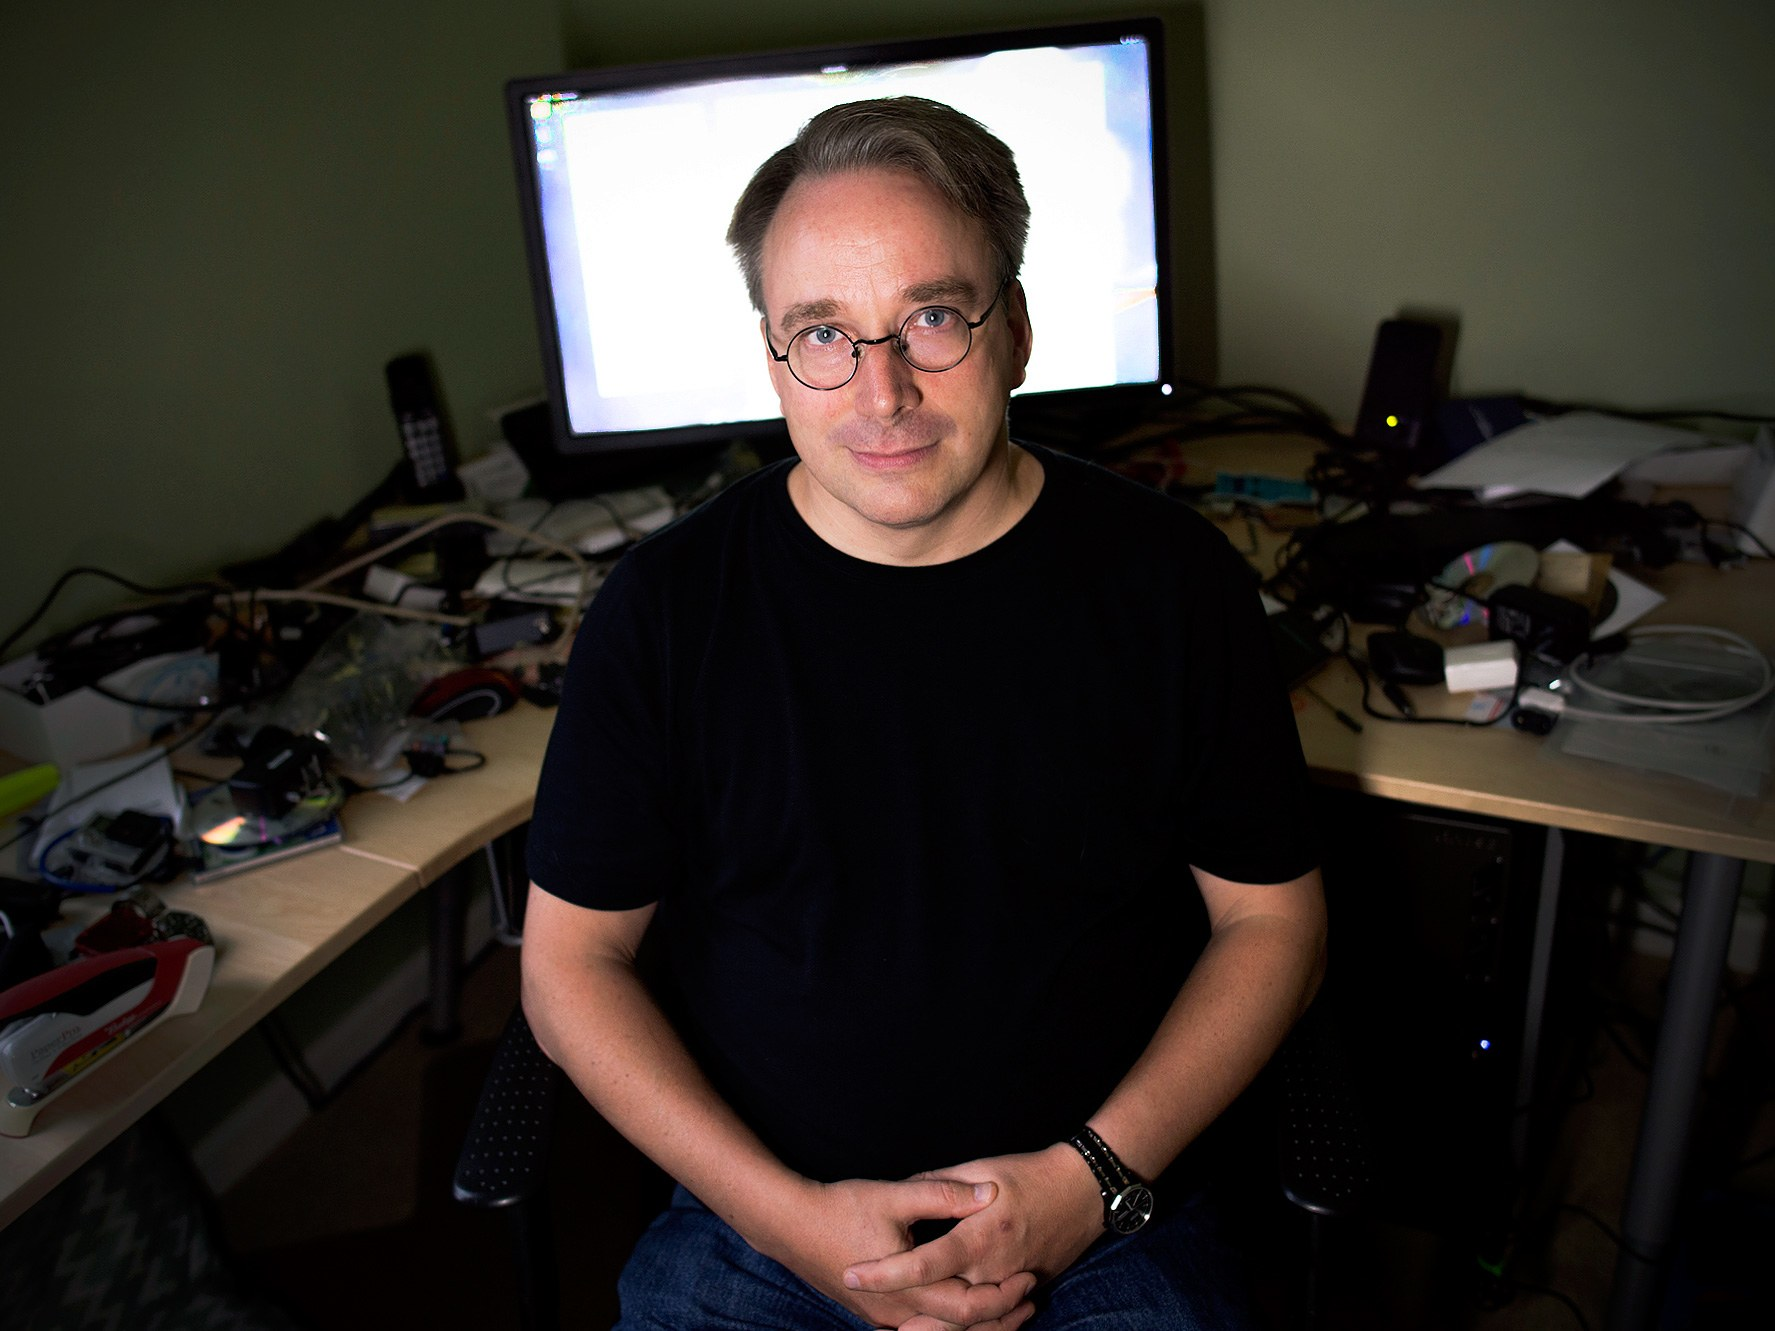
\includegraphics[width=\textwidth]{figures/linus.jpg}
            \end{figure}
        \end{columns}



    \end{frame}

    \section{GitHub}\label{sec:github}
    \begin{frame}{GitHub}
        \begin{columns}
            \column{0.5\textwidth}
            \begin{itemize}
                \item \url{https://github.com/}
                \item Central repository sharing
                \item Public and private options
                \item Project management
            \end{itemize}

            \column{0.5\textwidth}
            \begin{figure}
                \centering
                
\includegraphics[width=\textwidth]{figures/Octocat.png}
            \end{figure}
        \end{columns}

        \begin{alertblock}{Be mindful of privacy!}
            Never store sensitive information in git! There are better solutions for managing passwords, encryption keys, or other sensitive information.
        \end{alertblock}
    \end{frame}

    \begin{frame}{Creating an Account}
        Navigate to \url{https://github.com/}

        \begin{figure}
            \centering
            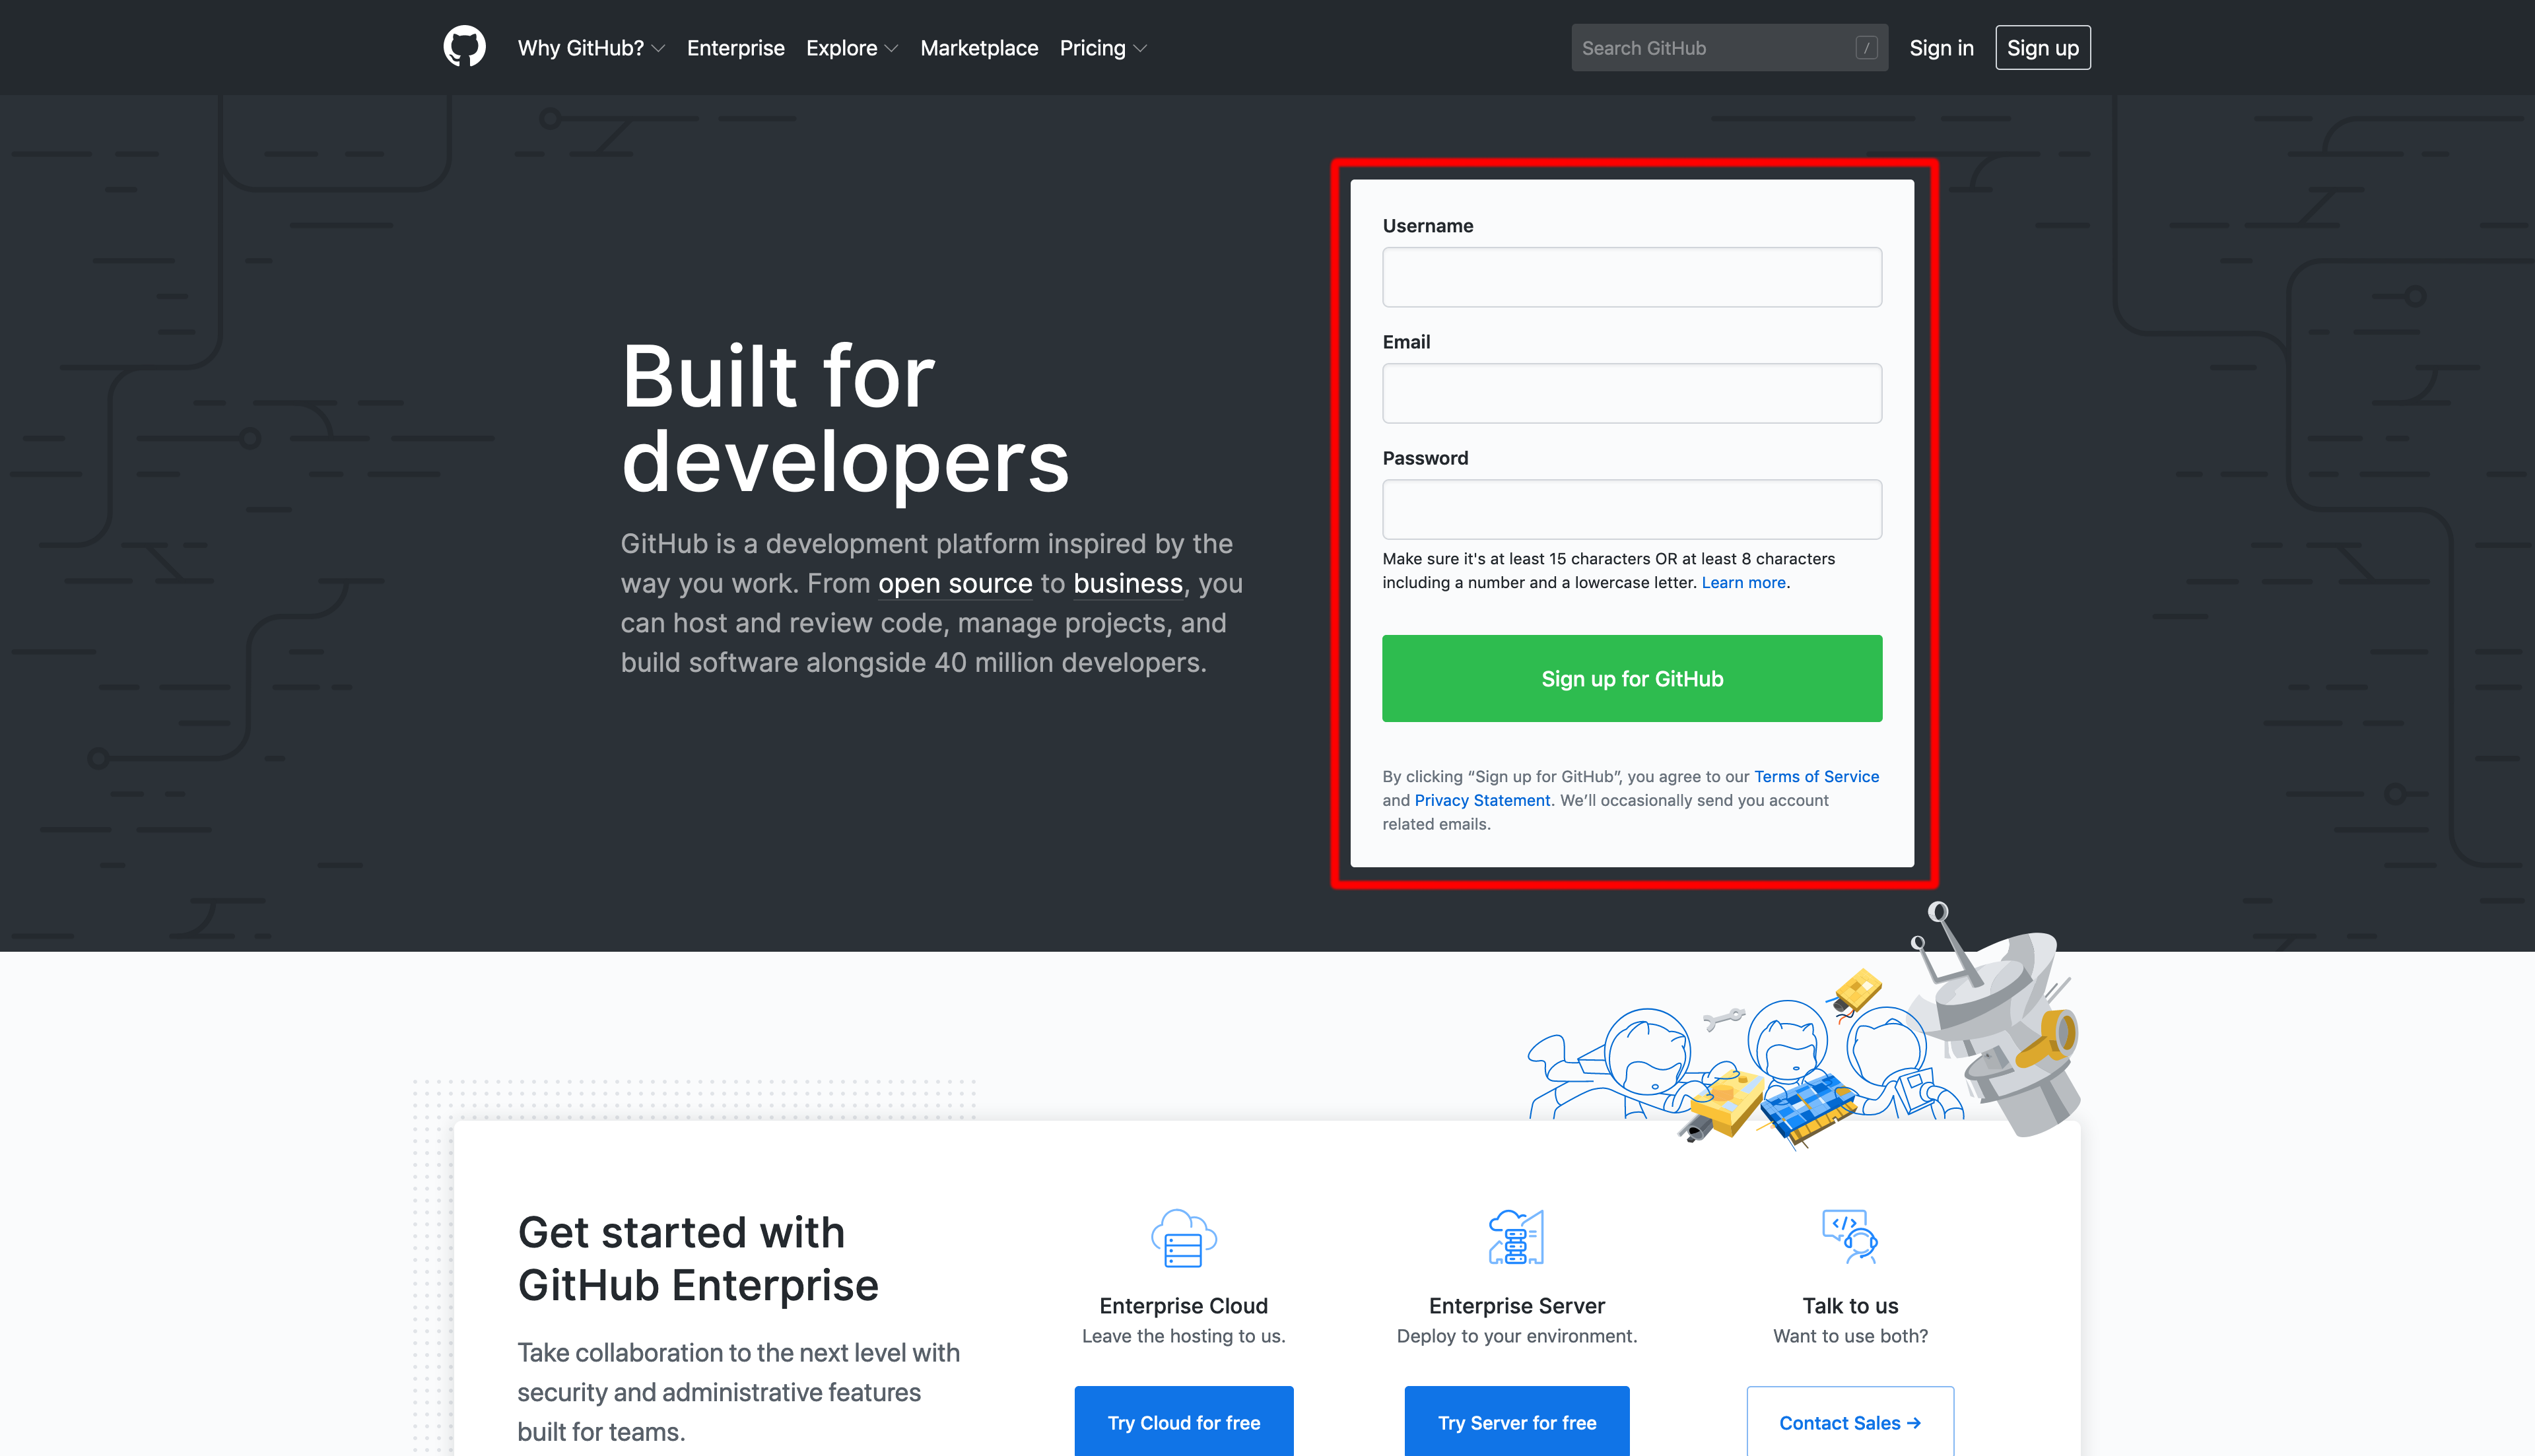
\includegraphics[width=\textwidth]{figures/github.png}
        \end{figure}
    \end{frame}

    \begin{frame}{Creating a Repository}
    \end{frame}

    \section{GitHub Desktop}\label{sec:github-desktop}
    \begin{frame}{GitHub Desktop}
        \begin{itemize}
            \item Cross-platform, open-source git client
            \item Graphical interface to most of git's features
            \item
        \end{itemize}
    \end{frame}

    \begin{frame}{Cloning a Repository}
    \end{frame}

    \begin{frame}{Upload an Existing Repository}
    \end{frame}

    \begin{frame}{Getting Changes}
    \end{frame}

    \begin{frame}{Adding Changes}
    \end{frame}

    \begin{frame}{Merge Conflicts}
    \end{frame}

    \begin{frame}{Branches}
    \end{frame}

    \begin{frame}{.gitignore}
    \end{frame}

    \begin{frame}{Project Management}
    \end{frame}

    \begin{frame}{Quick Review}
    \end{frame}

    \begin{frame}{Resources}
    \end{frame}

    \begin{frame}{Thank You!}
    \end{frame}


\end{document}